\documentclass{standalone}
\usepackage{tikz}

\begin{document}

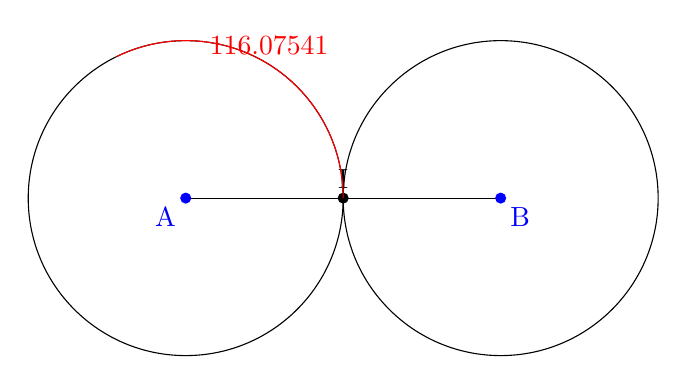
\begin{tikzpicture}[scale=2]
    % Define coordinates
    \coordinate (A) at (-1, 0);
    \coordinate (B) at (1, 0);
    \coordinate (I) at (0, 0);

    % Draw circles
    \draw (A) circle (1);
    \draw (B) circle (1);

    % Draw line segments
    \draw (A) -- (B);
    \draw (I) -- (A);
    \draw (I) -- (B);

    % Label points
    \fill[blue] (A) circle (1pt) node[below left] {A};
    \fill[blue] (B) circle (1pt) node[below right] {B};
    \fill[black] (I) circle (1pt) node[above] {I};

    % Label angle
    \draw[red] (I) arc (0:116.07541:1) node[midway, above] {116.07541};
\end{tikzpicture}

\end{document}